\documentclass{article}
\usepackage{amsmath}
\usepackage{graphicx}
\usepackage{float}
\usepackage{longtable}
\usepackage{hyperref}
\graphicspath{ {./images/} }

\title{Benchmarking the Internet Computer}
\date{2023-02-13}
\author{Douglas Bouchet}

\begin{document}
\pagenumbering{gobble}
\maketitle
\newpage
\pagenumbering{arabic}

\tableofcontents

\newpage
\section{Abstract}
This paper presents a study on the use of blockchain technology as a platform for performing heavy computational tasks
such as machine learning. Through a series of tests, the paper attempts to identify the capabilities of blockchain for
such applications. The results of the research indicate that the size of transactions is limited to ten thousand
and that there is a trade-off between redundancy and pace of execution. Furthermore, the length of the model has an
influence on the pace of the model. These results provide insights into the potential of blockchain for heavy
computational tasks and can be used to inform future research and development in this area.
\newpage
\section{Introduction}
The emergence of blockchain technology and its associated smart contracts has revolutionized the way we think about data
storage and computing. As a (student) researcher interested in the potential of blockchain technologies, I sought to explore the
ability of blockchain to provide a transparent and secure environment for performing heavy computational tasks, such
as machine learning. This paper aims to investigate if blockchain can indeed be used for such purposes.
In order to see if the blockchain can then be used to help with heavy computational tasks, we will take an already
existing protocol to perform this task, the Federated Learning. We will then see how it is possible to modify it by adding the blockchain.
We will detail the smart contracts used, as well as the interactions between the different agents involved in the
machine learning task. Finally we will test our new framework using diablo, a program that allows to submit transactions
to a blockchain, and to measure the performance of the latter, in response to these transactions. For more realism,
 the nodes constituting our blockchain will be emulated using machines made available by the AWS service

DO we add these ? -------
The expectations of some fundation such as Dfinity project
Can be questionable, as performaces of some BC can be quite limited
--------------
\section{Method}
\subsection{The need for computational resources in Machine Learning}
Recently, many machine learning models have been published. These models have become very popular mainly due to their
performance. We can quote models such as DALL-E, or GPT-3. The training of these models requires a huge amount of data
and computing power. If we wanted to train GPT-3 using one of the most powerful GPUs currently available,
the NVIDA v100, the time required would be about 300 years (also making the optimistic assumption that all the
training data could fit in the GPU RAM). There is therefore a need for techniques to increase computing power in order
to generate these huge models.
\subsection{The three main goals of scaling up the computational power}
When designing a system able to provide such an increase of power, the following three aspects should be taken care of
by this system, as they are the ones that make it currently feasible.
\begin{enumerate}
    \item \textbf{Provide reasonable performances}. Indeed, the purpose of such a system is to provide an increase in computing
     capacity. The availability of sufficient computing power is therefore one of the main factors.
    \item \textbf{Reward those that participates in the system}. What would be the interest for the participants to work for
     free, or without guarantee of payment?
    \item \textbf{Shouldn't be specific to machine learning}. This system should be able to adapt to any type of task, so as not
     to be too specific, and potentially limited in its evolution or adaptation.
\end{enumerate}

\subsection{Federated Learning, an existing system to provide computational resources}
Federated Learning is a system that allows to involve multiple devices in the training of a model. The idea is to
distribute the training data to the different devices, and to train the model on each of them. The model is then
aggregated to obtain a single model. This system is therefore able to provide a significant increase in computing power.
In this project, we will consider a simplified version of federated learning. We assume that each participants
already has the data needed to train the model. Our version consists of the following steps:
\begin{enumerate}
    \item The model is initialized on the server
    \item The model is sent to each participant
    \item Each participant compute one model update
    \item Each participant send the updated model to the server
    \item The server update the model using some aggregation rules
    \item Repeat step 2 to 5 for a given number of iterations, or until some convergence criteria is met
\end{enumerate}
This system has some limitations, such that the rewarding of the participants is not guaranteed, or the possibility for
new participants to join the process.
\subsection{Advantages of using a blockchain to enhance this protocol}
Using a blockchain to coordinate workers brings several advantages, which might help to solve the three main goals of
scaling up the computational power.
\begin{enumerate}
    \item Goal 1 "provide reasonable performances": Using a blockchain allow in theory anyone to join the learning
process. This can provide an unbounded increase in computing power. The only limitations would be the number of workers
involved in the learning, their power, but also the maximum number of participant the blockchain could handle.
    \item Goal 2 "reward those that participates in the system": Using a blockchain provide an easy way to reward the
participants. In order to to so, we could use smart contract, paying in gas participants that did a correct job - i.e
learn a correct model. This has the advantage that anyone could actually see the code executed when rewarding the
participants, as the smart contract code can be read from the blockchain. This is a very important point,
as it can bring confidence to the participants, increasing the trust in the system, and potentialy motivate participants
to join the process.
    \item Goal 3 "shouldn't be specific to machine learning": Redundancy protocol in blockchain is a measure taken to
ensure the continuity of the blockchain network by replicating the data across multiple nodes. This is done to ensure
that if one node fails, the data on the other nodes can be used to prevent any disruption to the network. This also
guarantee that data cannot be tampered. This implies that using a blockchain in combination with federated learning
isn't only reserved to machine learning problem, but any other type of problems, involving heavy computational tasks.
\end{enumerate}

slides which answer the 3 goals
\subsection{Including BC in federated learning, a naïve approach}
Now let's see how we can add a blockchain to our current federated learning protocol. The base case is the same as in
the federated learning scenario, but now we can add a smart contract between the server and the participants. The smart
contract is published by the server on the blockchain, and it will coordinate the participants. Our new protocol in
order to do one model update is the following:
\begin{enumerate}
    \item Server sends the model weights to the smart contract
    \item The smart contract sends the same model weights to a pool of participants choosen among all participants. The
number of participants in the pool (the ones that will perform the same model update) is called the \textbf{redundancy}
    \item By assumption, each participant has the training data, so each one can perform one model update
    \item Each participant send the updated model weights, along their public key to the smart contracts. The public key
is sent as the smart contract need to associate each model submission to a worker in order to potentially pay them later.
    \item The smart contract then set the elected model as the model with the most bids from participants.
    \item The elected model is then sent to the server, which can update its current model. This makes one epoch
    \item The steps 1 to 6 are then repeated for a chosen number, or until some convergence on loss is reached.
\end{enumerate}
This explanation was focus on only one pool/group of participants, but in a real case there would be several pools
running in parallel, allowing for a quicker model training, which is what this protocol is aiming at.\\
There is however a big problem with this protocol. As the smart contract is located on a blockchain, everything that is
actually written to the smart contract, can be read by anyone (assuming we are using a public blockchain). This means
that it is actually possible for a participant to not actually perform the model update, but still get paid. Let's
illustrate this with a simple example.\\
Suppose we have a worker($W_0$) that sends its updated model weights $M_{W_0}$to the smart contract. The transaction would then
be ($M_{W_0},Pk_0$). Some evil worker ($W_1$) can read this transaction, and steal the model weights $M_{W_0}$. It can then send
the following transaction ($M_{W_0}, Pk_1$). The smart contract has no way to know if the model weights $M_{W_0}$ were actually
learned by $W_0$ and $W_1$. If this model is the elected one, then both $W_0$, $W_1$ will be paid. Indeed it's actually
possible for someone to get paid, without performing the computation. Let's now see how we can solve this issue.
\subsection{Solving the model stealing issue}
In order to solve the model stealing issue, we will use a \textbf{commit-reveal} protocol. It involves two steps:
a sender first commits to a message by providing a cryptographic hash of it, without revealing the actual message.
Then, the sender reveals the message to prove they are the one who committed to it.\\
Let $H$ be a one-way cryptographic hash function. This involve that it is easy to compute $H(x)$, but it is hard to
compute $x$ from $H(x)$.\\
Our commit-reveal schema will be the following:
\begin{itemize}
    \item Commit: the worker $W_i$ sends $H(M_{W_i}|Pk_i)$ to the smart contract
    \item Reveal: the worker $W_i$ sends $M_{W_i},Pk_i$ to the smart contract
\end{itemize}
After the reveal, the smart contract can check that $H(M_{W_i}|Pk_i)$ is equal to the commit. If it is the case, then
the submission is considered valid. Otherwise its rejected. The elected model is computed on valid submission only.\\
One important thing to add: during the reveal phase, no more commits are accepted as during the reveal we send
the model in clear. If new commits were still accepted, it would be possible for someone to read some of the submitted
models, and create a commit with them. The commit would indeed be valid, therefore our protocol wouldn't prevent anymore
from model stealing.
\subsection{Dealing with smart contract limited memory}
- soem numbers for max var size
- idea: split the models
In order to deal with these limitations, we will not send the model weights in one transaction during the reveal phase,
but rather send chunks of it. Now suppose that we can write our model as following:
\begin{equation}
    M = M_1 | M_2 | ... | M_n
\end{equation}
We modify the reveal as following:
\begin{enumerate}
    \item worker i sends $H(M_{W_{i, 1}})$, which is the hash of the first chunk of the model
    \item he can then send the hash corresponding to the next chunk: $H(M_{W_{i, 2}})$ and so on.
\end{enumerate}
The smart contract create only one variable for the chunk received (for each worker). This variable contains the hash
of the first chunk, which is computed by the smart contract. The model chunk can be stored on an external storage, to
not use memory in the smart contract. Upon receiving the next chunk,
it update the previous hash by hashing it with the new chunk. The new chunk is also added to the external storage. This
operation is repeated for every new chunk received from this worker. The last chunk received is also concatenated with
the public key of the worker.\\
At the end, for each worker we have the complete model in an external storage, and the following hash on the smart contract
\begin{equation}
    \begin{split}
         Hash_{W_i} & = H(...(H(H(M_{W_{i, 1}})|M_{W_{i, 2}})|...)|M_{W_{i, n}}|Pk_i) \\
         & = H(M_{W_{i, 1}} | M_{W_{i, 2}} | ... | M_{W_{i, n}} | Pk_i) \\
         & = H (M_{W_i} | Pk_i)
        \end{split}
\end{equation}
The second line is obtained using the Merkle-Damgard theorem. We see that using this construction
$Hash_{W_i}$ during reveal protocol can be compared to the one send during the commit protocol. \\
We don't need to modify the commit, as we only send an hash, which is of small constant size. Using this construction,
we can therefore reduce the memory used on the smart contract. In fact, we are only storing hash on the smart contract,
which are 32 bytes long.
- total expected memory usage on the smart contract
\section{Learning a model using blockchain result and observations}
Now that we have seen a theoritical protocol that would allow to train a machine learning model.
In order to measure the performances of our protocol, we will simulate a Quorum blockchain using Amazon Web Service. TODO check name
The nodes which are responsible of validating the transactions, will be rented on AWS. Each one has two virtual cpu, and
four Gb of RAM. There are eight such nodes, all located in the same geographical region (Paris). We implemented the
smart contract responsible for all the methods defined in {3.5, 3.6, 3.7} in solidity. Diablo will be used to send
transactions. This is a tool that given a list of transactions defined by the smart contract method
called, the arguments passed to the fonction and the time where the transaction should be send, will send them to the
smart contract. With this technology, we can easily modify the 'workload' (sequence of transaction) we will be sending
to the smart contract. This will be usefull when varying the number of transactions send by second.
- small intro about aws + diablo
\subsection{First limitation, transaction size}
One first problem to deal with when working with blockchain is the transaction size. In fact, we should expect
transaction with a high number of parameters take more time and ressources to be handled than smaller transactions. This
can impact the throughput our blockchain is able to handle.\\
Let's start by tuning the transaction size. In the following experiment, we will be calling a smart contract function
that only copy uint256 (256 bits unsigned integers) inside an array. For each array size ranging from one thousand
to fifty thousand, we will send one hundred transaction per second during twenty second. We then measure which percentage of transactions were committed. In order to have more robust
results, we will perform twenty measurements on each array size. We plot our results on the graph below.
\begin{figure}[H]
    \hspace*{-1.55cm}
    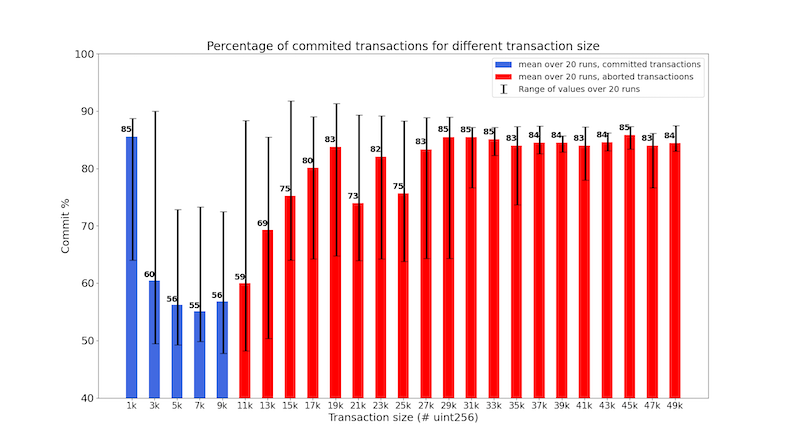
\includegraphics[scale=0.75]{max_array_length}
    \hspace{2mm}%
    \caption{Tuning the transaction size}
\end{figure}
There are two phases on the graph. During the first blue one we see that as the transaction size increases, the percentage of committed transaction decreases. This is an expected result, as the more parameters we have, the more time it takes to process the transaction. In the second phase in red, we can see that the percentage of commited transaction actually increases with their size, until 85\% of commit. This counter intuitive results is due to the fact that transctions with too much parameters aren't processed by the blockchain. In fact, nodes handling them run out of gas before finished to fill the array. In consequence, the transactions are aborted, and therefore not persitted to the blockchain. This can greatly impact the throughput of the blockchain, as it takes resources to actually persist the transaction. In diablo an aborted transaction is considered as a commit. This explains why we obtain this graph shape. We can deduce that we shouldn't use transactions of more than ten thousands parameters, as going beyond indude lots of aborted transactions.

\subsection{The Redundancy/Pace trade-off}
Remember from section 3.7 that participants are sending chunks of the model. The pace is the time each participant is
waiting between sending two chunks. The redundancy is the number of participants that will be asked to do the same
computation. We will now see if there is a trade-off between the pace and the redundancy. We did the following experiment:
we learned a one million parameters model, but only for one epoch as it can took already one hour to perform one epoch with
this model length. We vary the redundancy and the pace. On the graph below is plotted for each
redundancy the minimum pace that is required to have at least eighty five percent of committed transactions. We took
eighty five as a threshold because this indicates that most of the transactions have actually been committed, which
means that the model has chances of being learned. From our result of previous section about tuning the
transaction size, we decided to use chunk of size one thousand.
\begin{figure}[H]
    \hspace*{-2cm}
        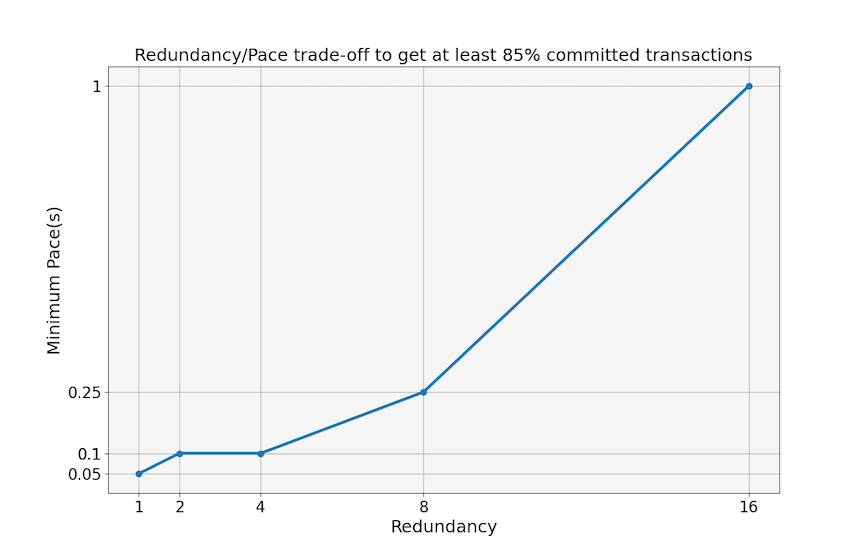
\includegraphics[scale=0.75]{redundancy_pace}
    \hspace{2mm}%
    \caption{Redundancy/Pace trade-off}
\end{figure}
We can observe that as the redundancy increases, the minimum pace also increases. This is due to the fact that we are
involving more participants in the process. As each participants needs to send all its model's chunks, we have to
increase the time each participants wait between sending each chunk in order to not overload the blockchain with
too much transactions. We can see that there is a trade-off between the redundancy and the mininum pace. This means
that the more secure the learning has to be, the more time is needed to perform this learning, as we need to increase
the mimimum pace.
\subsection{Minimum pace depending on model length}
Now that we have seen that there is a trade-off between the redundancy and the pace, we will try to give an idea of the
minimum pace needed to learn a model of a given length. This could give a rough idea of how much training time would be
expected using our proposed framework. In the following experiment, we repeated what was done in previous subsection,
but we varied the model length, instead of fixing it to one million. We also vary the pace, and seted the minimum one leading
to at least eigty five percent of committed transactions to be the minimum pace. We however fixed the redundancy to eight. We choosed eight as
the redundancy used by the DFINITY fundation is less than $\frac{1}{3}$ \cite{DFINITY_redundancy} of the workers.
\begin{figure}[H]
    \hspace*{-2cm}
        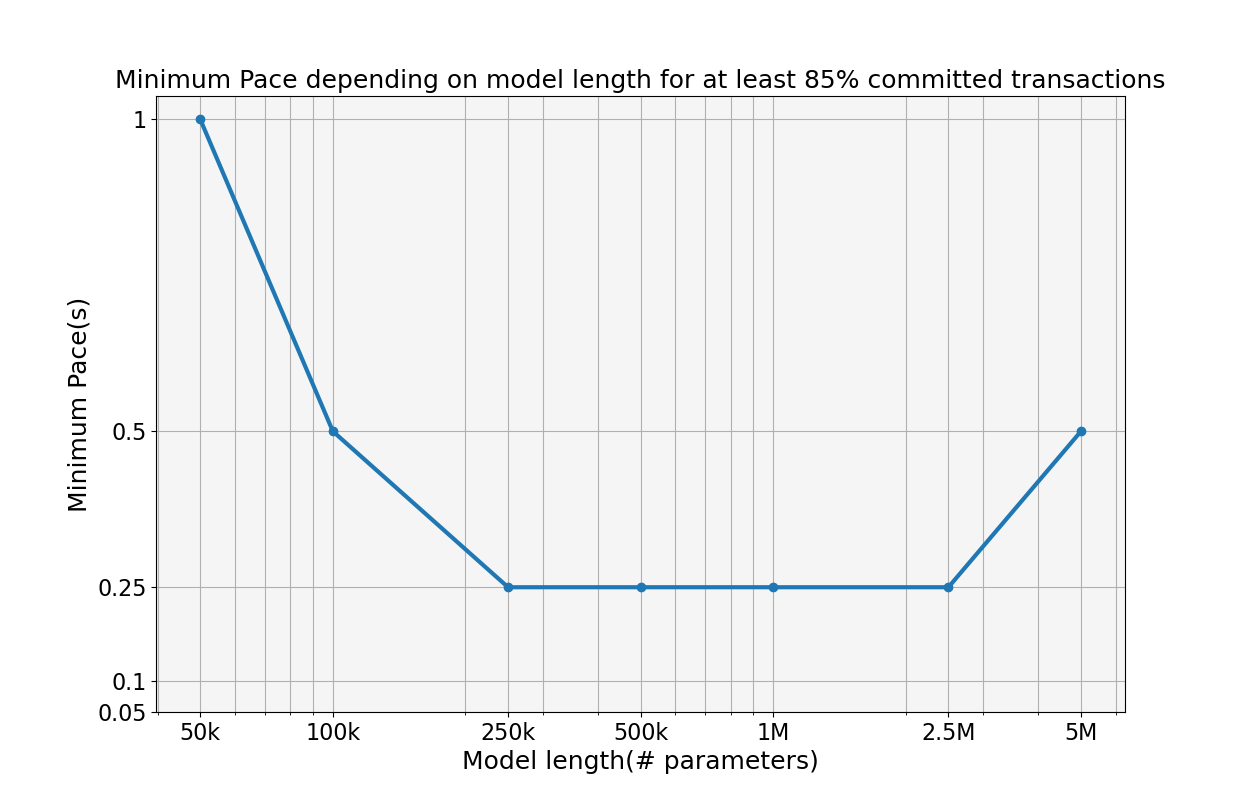
\includegraphics[scale=0.5]{length_pace}
    \hspace{2mm}%
    \caption{Minimum pace as a function of model length}
\end{figure}
From the following graph, we can see that when increasing the model length from fifty thousand to two hundred
fifty thousand, we can actually reduce the minumum pace. This might be due to the fact that in the first phase of the
learning, all the participants send the hash of their model, almost all at the same time. The blockchain might be overloaded
and would need some time to handle those transactions. Using a higher model length would ensure that we have such a time.
Then from two hundred fifty thousand to 2.5 million, we see the minimum pace being actually flat to 0.25 seconds. This is an expected result
as increasing the model length doesn't increase the number of transactions per second. It only increases the time needed to
send all the chunks, are there are more of them. Finally, from 2.5 million to 5 million, we see the minimum pace increasing.
This is a strange result, as we wouldn't expect it. This could be due to some network congestion appening after some time,
but a more in depth analysis would be needed to confirm this hypothesis. One could also monitor the nodes of the blockchain,
in order to see if they're actually overloaded. This could give a better idea of what is happening.
\subsection{Expected training time for some classical models}
Now that we know the minimum pace used to train models of a length around one million parameters, we can estimate
how much time we would need to actually train some real models. In the following results, we make the
assumption that model with a length higher than 2.5 million parameters can be trained with a pace of 0.25 seconds. We've
however seen from previous section that it doesn't seems to be the case, and these results would rather be lower bound.
\begin{longtable}{|l|l|l|}
    \hline
    Model                                & Number of epochs & Training Time \\ \hline
    \endfirsthead
    %
    \endhead
    %
    CNN for MNIST (1 million parameters) & 100              & 7 hours       \\ \hline
    BERT (100 million parameters)        & 100 000          & 8 years       \\ \hline
    GPT-3 (175 billion parameters)       & 10 000           & 1400 years    \\ \hline
\end{longtable}
Training a CNN for MNIST take twenty minutes\cite{MNIST_runtime} on a mac book . We however see that it takes seven hours
with our implementation, which is quite a huge loss of performances. For BERT, it would take several days \cite{BERT_runtime} using one of the
most powerfull GPU. Again we see that our framework would need at least height years to do the training. Finally, for GPT-3,
it would take 1400 years to train it using our framework. Some estimation of the training time for GPT-3 using powerfull
GPU can be found in \cite{GPT_runtime}. They estimate the training time to be 665 years. We only see a two times
factor, but our estimate of 1400 years was optimal, and may not have taken into account several other parameters that could influence
the training time (such as GPU memory limitation). To conclude we have seen that using this framework allowing to use the
blockchain to help in machine learning induce a huge loss of performances. Again in our computation, we only estimate the
training time as the time we need to send all the model's chunk hash to the smart contract. We didn't take into account
the training time of the participants to actually compute the new model weights.
\section{Conclusion}
During this project, we have seen that it can be possible to use the blockchain to help in heavy computational tasks, such as
machine learning. We have defined a framework allowing to do so, and have seen that it is possible to use it to train a model.
We have however seen that there are several challenges to overcome in order to make this framework usable in real life.
We focused on the Quorum blockchain, but there might be other blockchains allowing a higher transaction throughput, or size.
We also saw that there is a trade-off between the redundancy and the minimum pace. Finally we provided lower bounds
on the training time for some classical models.\\
Focusing on smaller machine learning model could be a good application for our framework as it could invoke a smaller workload
on the blockchain. The framework might also be explored for other tasks in machine learning such as the transfert learning, This is a method where
you use an already trained model, and vary only some of its parameters in order to specialize it to a new task. This has the
advantage of using a lower number of parameters, and could in consequence have a good synergy with our framework.\\
You can find the code we used for this project \href{https://github.com/douglasbouchet/ml_on_blockchain}{on github.}


\begin{thebibliography}{9}
    \bibitem{DFINITY_redundancy}
    2022, \href{DFINITY white paper}{https://internetcomputer.org/whitepaper.pdf} 2.2 Consensus layer

    \bibitem{MNIST_runtime}
    Mustafa Hoda (2018) \href{https://medium.datadriveninvestor.com/my-take-at-the-mnist-dataset-97304dff2057}{https://medium.datadriveninvestor.com/my-take-at-the-mnist-dataset-97304dff2057}

    \bibitem{BERT_runtime}
    Aditya Bindal, Kevin Haas, and Indu Thangakrishnan (2019) \href{https://aws.amazon.com/fr/blogs/machine-learning/amazon-web-services-achieves-fastest-training-times-for-bert-and-mask-r-cnn/}{https://aws.amazon.com/fr/blogs/machine-learning/amazon-web-services-achieves-fastest-training-times-for-bert-and-mask-r-cnn/}

    \bibitem{GPT_runtime}
    Chuan Li (2020) \href{https://lambdalabs.com/blog/demystifying-gpt-3}{https://lambdalabs.com/blog/demystifying-gpt-3}, Training the Model

\end{thebibliography}
\end{document}
